\section{Including title, author and date information}

Adding a title, author and date to our document requires three more lines in the \emph{preamble} (not the main body of the document). Those lines are:

\begin{itemize}
    \item \verb|\title{My first LaTeX document}|: the document title
    \item \verb|\author{Hubert Farnsworth}|: here you write the name of the author(s) and, optionally, the \verb|\thanks| command within the curly braces:
    \begin{enumerate}
        \item \verb|\thanks{Funded by the Overleaf team.}|: can be added after the name of the author, inside the braces of the author command. It will add a superscript and a footnote with the text inside the braces. Useful if you need to thank an institution in your article.
    \end{enumerate}
    \item \verb|\date{August 2022}|: you can enter the date manually or use the command \verb|\today| to typeset the current date every time the document is compiled
\end{itemize}

With these lines added, your preamble should look something like this:

\begin{tcolorbox}
\begin{verbatim}
    \documentclass[12pt, letterpaper]{article}
    \title{My first LaTeX document}
    \author{Hubert Farnsworth\thanks{Funded by the Overleaf team.}}
    \date{August 2022}
\end{verbatim}
\end{tcolorbox}

To typeset the title, author and date use the \verb|\maketitle| command within the \emph{body} of the document:

\begin{tcolorbox}
\begin{verbatim}
    \begin{document}
    \maketitle
    We have now added a title, author and date to our first \LaTeX{} 
    document!
    \end{document}
\end{verbatim}
\end{tcolorbox}

The preamble and body can now be combined to produce a complete document which can be opened in Overleaf:

\begin{tcolorbox}
\begin{verbatim}
    \documentclass[12pt, letterpaper]{article}
    \title{My first LaTeX document}
    \author{Hubert Farnsworth\thanks{Funded by the Overleaf team.}}
    \date{August 2022}
    \begin{document}
    \maketitle
    We have now added a title, author and date to our first \LaTeX{}
    document!
    \end{document}
\end{verbatim}
\end{tcolorbox}

This example produces the following output:

\fbox{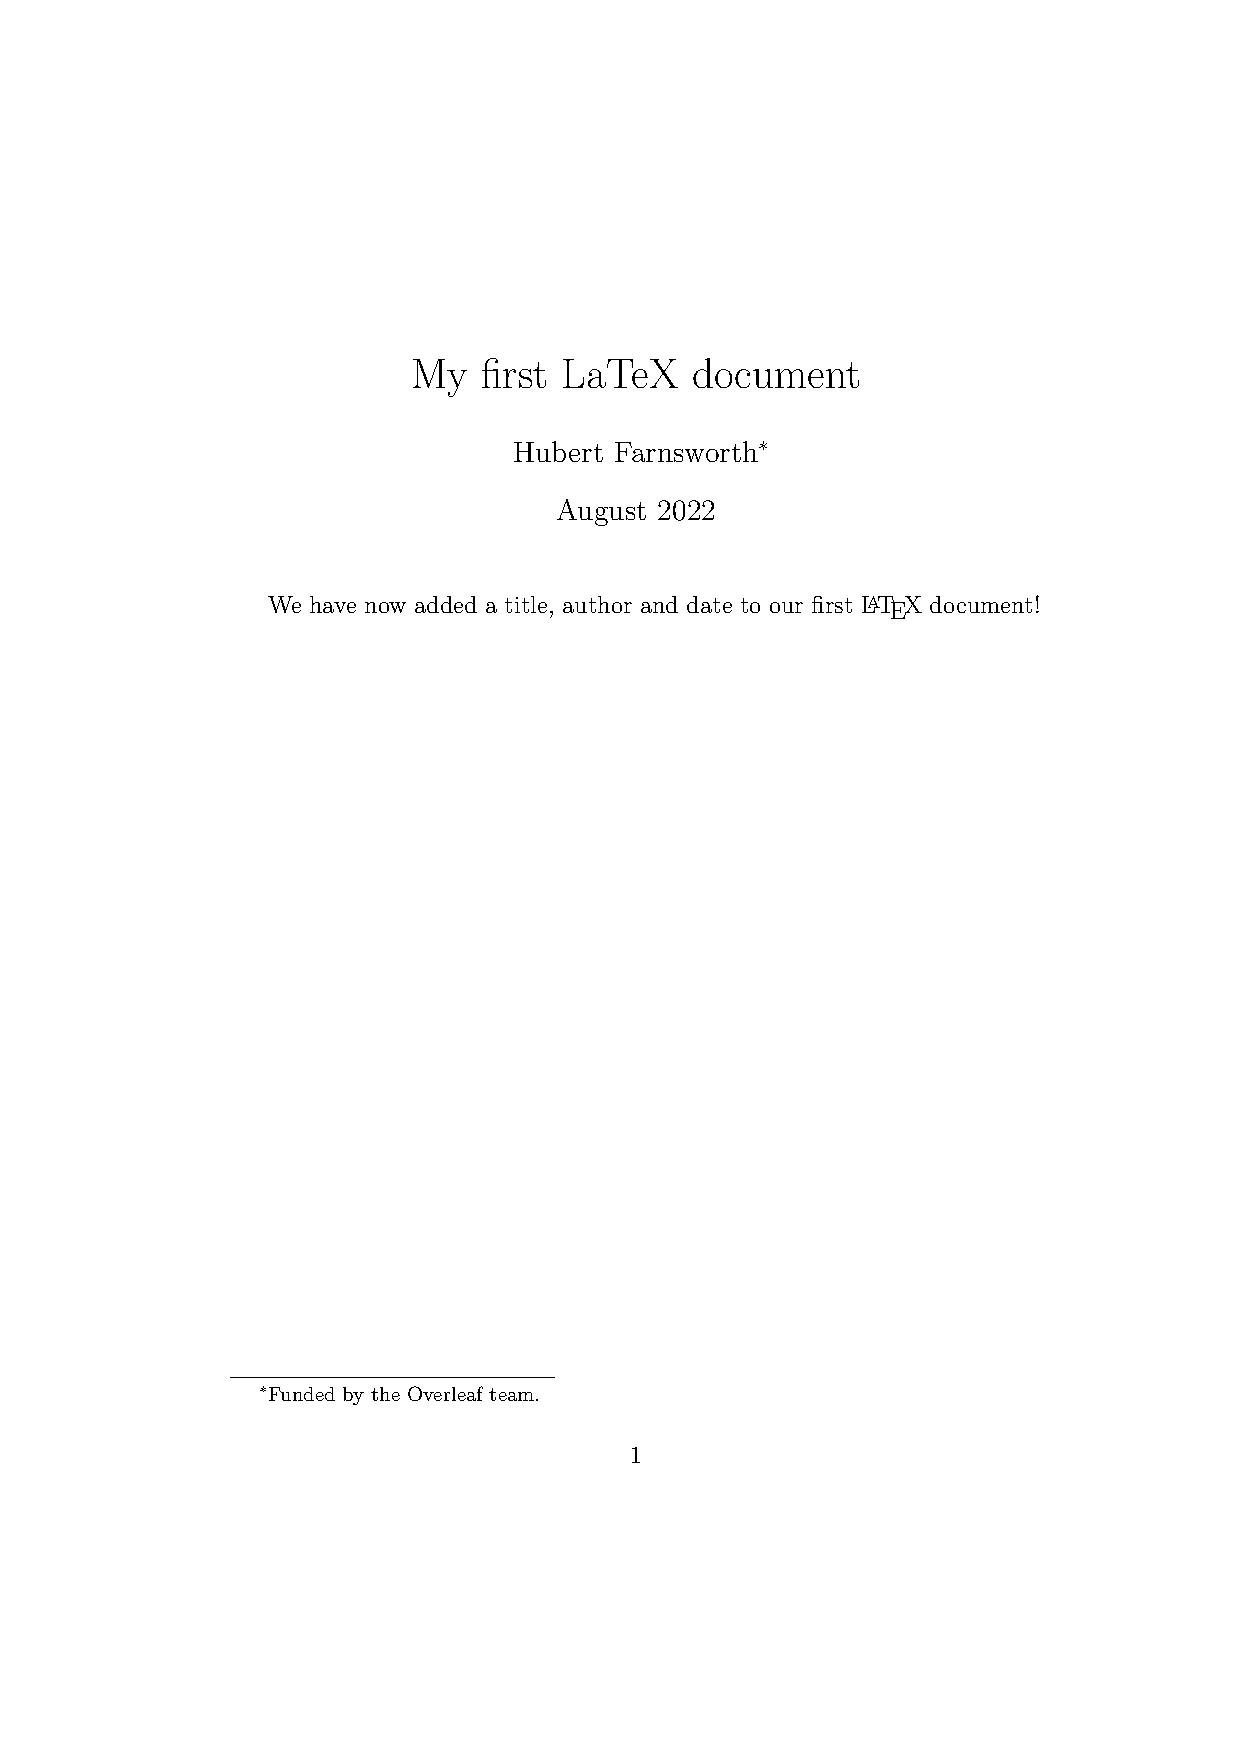
\includegraphics[width=\textwidth]{Example 5-1.pdf}}